\section{Methods}
\label{sec:methods}

\subsection{Logistic Counterexample}
\label{sec:logistic}

\paragraph{Construction.}
Let $x=\epsilon s$, $y^*=\mathbf1\{x>0\}$, with magnitudes
$s\in\{1,L\}$ of probabilities $\rho_1=1-b$, $\rho_L=b$,
$L\geq1$, $0<b<1$, and independent equiprobable sign $\epsilon\in\{-1,+1\}$.
The learner samples $\hat y\sim\operatorname{Bernoulli}(\sigma(\theta x))$,
where $\sigma(z)=(1+e^{-z})^{-1}$. Correctness is $p_s=\sigma(s\theta)$
for either sign, giving
\begin{equation}
 P(\theta)=\sum_s\rho_s p_s,\qquad
 P'(\theta)=\sum_s\rho_s s p_s(1-p_s)>0.
 \label{eq:sampling-accuracy}
\end{equation}
This is sampled-label accuracy, not greedy classification. The two group
identities remain distinct in the $L=1$ ablation.

Both rules accept correct candidates with probability $a$. $R$ accepts errors
with probability $b$; $S$ prefers the large group at the same error mass.
Set $m_s=\rho_s(1-p_s)$, $Q=b(m_1+m_L)$, and
\begin{equation}
 \begin{aligned}
 r_{R,s}&=b, &r_{S,L}&=\min\{1,Q/m_L\},\\
 &&r_{S,1}&=\max\{0,Q-m_L\}/m_1.
 \end{aligned}
 \label{eq:structured-rule}
\end{equation}
At finite $\theta$, denominators are positive. Both rules have TPR $a$,
FPR $b$, and, at a common $\theta$, $Z=aP+b(1-P)$, $\pi=aP/Z$.
The stopped-gradient binary-cross-entropy gradient is
\begin{equation}
 g_v(\theta)=\frac{\sum_s\rho_s s p_s(1-p_s)(r_{v,s}-a)}
 {aP(\theta)+b(1-P(\theta))}.
 \label{eq:logistic-gradient}
\end{equation}
Appendix~\ref{app:proof} derives this loss derivative with sampling and
acceptance held fixed.

\begin{lemma}[Piecewise acceptance and influence]
\label{lem:piecewise}
For $L>1$, $0<b<1$, and finite $\theta$, rule $S$ satisfies
\begin{equation}
 (r_{S,1},r_{S,L})=
 \begin{cases}
 (0,D/(1-p_L)),&\theta\leq0,\\
 (b(p_L-p_1)/(1-p_1),1),&\theta\geq0,
 \end{cases}
 \label{eq:piecewise}
\end{equation}
where $D=1-P$. Both expressions agree at zero. Consequently
$0\leq r_{S,1}\leq b$, and~\eqref{eq:logistic-gradient} holds for both rules.
\end{lemma}

\begin{proposition}[Matched rates with opposite initial updates]
\label{prop:separation}
Let $0<b<a<1$, $L>1$, $\theta_0=0$, and $\bar s=1-b+bL$. Then
\begin{equation}
 g_R(0)=\frac{(b-a)\bar s}{2(a+b)},\qquad
 g_S(0)=\frac{bL-a\bar s}{2(a+b)}.
 \label{eq:general-initial}
\end{equation}
The $R$ update improves sampling accuracy for every $\eta>0$; the $S$ update
harms it if and only if $L>a(1-b)/[b(1-a)]$.
At $a=3/4$ and $b=1/2$, the two rules have
$(\mathrm{TPR},\mathrm{FPR},Z,\pi)=(3/4,1/2,5/8,3/5)$, while
\begin{equation}
 g_R(0)=-\frac{L+1}{20},\qquad g_S(0)=\frac{L-3}{20}.
 \label{eq:initial-gradients}
\end{equation}
Thus $L>3$ yields opposite accuracy changes.
\end{proposition}

\begin{remark}[Magnitude contrast]
At $a=3/4,b=1/2$, $L=1$ gives equal gradients $-0.1$; at $L=2$,
both updates improve accuracy, and at $L=3$ the $S$ update is zero.
For $L=10$, $\Delta\theta_R=+0.55\eta$ and $\Delta\theta_S=-0.35\eta$.
These initial comparisons alone do not establish long-run separation.
\end{remark}

\begin{theorem}[Long-run separation under resampled population flow]
\label{thm:flow}
Let $0<b<a<1$ and $L>a(1-b)/[b(1-a)]$. Under candidate resampling and
acceptance probabilities recomputed at the current parameter, consider
$\dot\theta_v=-g_v(\theta_v)$ from $\theta_R(0)=\theta_S(0)=0$.
Both flows exist uniquely for all $t\geq0$. Then
\begin{equation}
 \begin{aligned}
 \theta_R(t)&\uparrow+\infty,&P(\theta_R(t))&\longrightarrow1,\\
 \theta_S(t)&\downarrow\theta_*<0,&P(\theta_S(t))&\longrightarrow P(\theta_*)<1/2,
 \end{aligned}
 \label{eq:flow-limits}
\end{equation}
where $\theta_*$ is the largest negative zero of $g_S$. TPR and FPR are
$(a,b)$ throughout both flows. Global uniqueness of the $S$ equilibrium is
not asserted.
\end{theorem}

\begin{corollary}[Non-identifiability from aggregate verification statistics]
\label{cor:nonidentification}
Even with the learner and initial candidate distribution fixed, no function
of $(\mathrm{TPR},\mathrm{FPR},Z,\pi,P_0)$ alone can determine the sign of
the next sampling-accuracy change for every acceptance rule. Identical
initial summaries can also precede the different limits in
Theorem~\ref{thm:flow}.
\end{corollary}

\begin{remark}[Yield after divergence]
TPR and FPR remain matched along diverging population flows, but yield and
precision generally differ. At $a=3/4$, $b=1/2$, and $L=10$, both start
at $(Z,\pi)=(5/8,3/5)$. Numerically, the $S$ flow converges to
$(Z_S,\pi_S)\simeq(0.590,0.457)$, whereas the $R$ flow reaches
$(Z_R,\pi_R)\simeq(0.719,0.915)$ at $t=20$.
Appendix~\ref{app:proof} gives further population readouts.
\end{remark}

\subsection{A Population Guarantee for Targeted Auditing}
\label{sec:audit-theory}

After selection by $S$, a perfect correctness oracle independently audits
each accepted $s=L$ candidate with probability $q\in[0,1]$. Audited errors
are removed; correct candidates and the $s=1$ group are unchanged.
The effective error rates are $\widetilde r_1=r_{S,1}$ and
$\widetilde r_L=(1-q)r_{S,L}$, and the gradient is normalized by the
\emph{post-audit} yield
$Z_q=aP+\sum_s\rho_s(1-p_s)\widetilde r_s$.

\begin{theorem}[Sharp uniform threshold for the specified audit policy]
\label{thm:audit}
For $0<b<a<1$ and every finite $L>1$, the audited population flow from zero
strictly improves $P$ and has $P\to1$ whenever $q\geq1-a$.
This threshold is sharp uniformly over $L$: for every $q<1-a$, choosing
\begin{equation}
 L>\frac{a(1-b)}{b(1-a-q)}
 \label{eq:audit-contrast}
\end{equation}
gives an initially harmful audited update and convergence to a negative
equilibrium with accuracy below $1/2$.
\end{theorem}
% Vector composition; original audit package remains unchanged.
\begin{figure*}[!t]
\centering
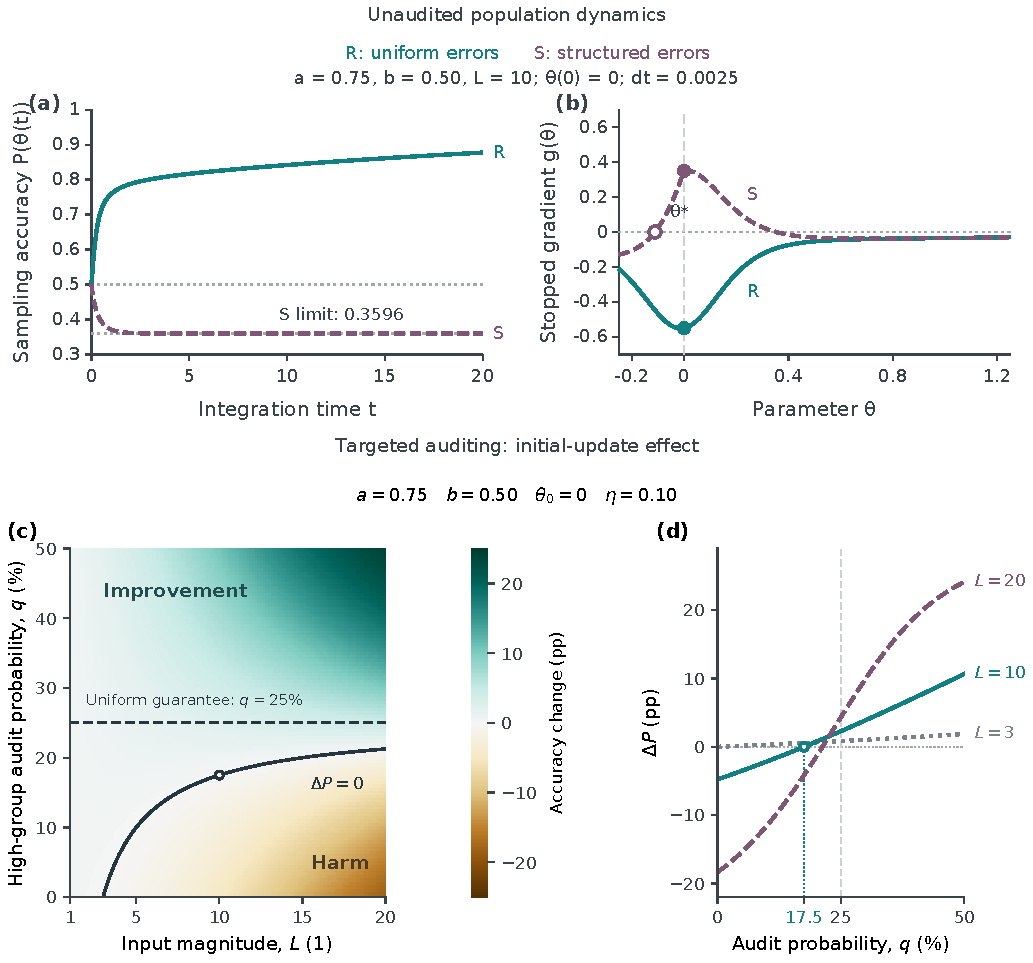
\includegraphics[width=0.6\textwidth]{figures/population_overview/population_overview.pdf}
\caption{Population dynamics and targeted auditing at $a=0.75$,
$b=0.5$, and $\theta_0=0$.
(a,b) Unaudited $R/S$ accuracy and gradients at $L=10$; filled/open
markers denote initial gradients/the negative $S$ equilibrium.
(c,d) Audited $S$ one-step change $100[P(-\eta g_{S,q}(0))-1/2]$ in
percentage points ($\eta=0.1$), with $L=3,10,20$ slices.
The solid boundary is $q_c(L)=0.25-0.75/L$ where nonnegative; the dashed
line marks the uniform flow threshold $q=0.25$ (Theorem~\ref{thm:audit}).
High-group query probability $q$ gives initial global query fraction
$B(q)=0.7q$. Panels (c,d) show initial updates, not convergence.
These are population calculations, not language-model measurements
(Appendix~\ref{app:numerical-readouts}).}
\label{fig:population-overview}
\end{figure*}


\paragraph{Initial-update illustration.}
Figure~\ref{fig:population-overview} illustrates the population flow and
initial-update boundary $q_c(L)=0.25-0.75/L$ at $a=3/4,b=1/2$.
For $L=10$, initial improvement requires $q>0.175$; the uniform flow
guarantee requires $q\geq0.25$. Initial-update readouts do not establish
convergence (Appendix~\ref{app:proof}).

\begin{corollary}[Vanishing global query fraction can suffice]
\label{cor:audit-budget}
At initialization, the expected fraction of the accepted pool queried by
this policy is $B(q)=qb(a+1)/(a+b)$. For fixed $a\in(0,1)$, taking
$q=1-a$, $b\downarrow0$, and
$L>a(1-b)/[b(1-a)]$ yields unaudited separation but audited convergence to
accuracy one, while $B(q)\to0$.
\end{corollary}
This family requires growing magnitude contrast. The threshold is not
minimax over policies: it assumes known groups, perfect queries, population
gradients, and fresh resampling, excluding the empirical policies in
Section~\ref{sec:budgeted-auditing}.

\subsection{Joint Subset Construction}
\label{sec:matching}

\paragraph{Controlled intervention.}
From each block's common pretraining pool, we select one response per retained
prompt in each arm, sharing prompts, correct-response IDs, $C:E=3:1$,
$K=C+E$, and unit weights. Graph supervised-token counts match exactly per
prompt (including EOS, excluding prompt/padding). Exact labels simulate noisy
acceptance; no LLM judge is used.

Each graph error-role prompt has an exact-length bucket containing a target
error and another signature. $R$ samples uniformly from that bucket; $S$
selects \texttt{nonshortest} errors. Arithmetic disables length matching
after failure throughout the ladder: $R$ samples all prompt errors and $S$
selects \texttt{ignore\_parentheses}. The intervention conditions on eligible
prompts and graph length buckets; coincident selections are retained.
Appendix~\ref{app:matching} gives role assignment and matching certificates;
Appendix~\ref{app:h100-results} reports feasibility.

\paragraph{Feasibility and matched quantities.}
The common size is the largest $K\in(64,32,16)$ feasible across a task
family's blocks; otherwise selection stops without seed or tolerance changes.
With correct/incorrect counts $N^+,N^-$ in the original nontruncated pool,
\begin{equation}
 \begin{aligned}
 \mathrm{TPR}_{\mathrm{final}}&=C/N^+,&
 \mathrm{FPR}_{\mathrm{final}}&=E/N^-,\\
 Z_{\mathrm{final}}&=K/(N^++N^-),&
 \pi_{\mathrm{final}}&=C/K.
 \end{aligned}
 \label{eq:finite-rates}
\end{equation}
These statistics agree across arms within a block, with precision $3/4$,
not the analytical $3/5$. Table~\ref{tab:subset-counts} gives downsize
counts and the guarantee's scope.

\subsection{One-Step LoRA and Diagnostics}
\label{sec:lora}

\paragraph{Update protocol.}
The one-step design freezes the base and uses LoRA~\citep{hu2021lora}:
rank $8$, $\alpha=16$, \texttt{q\_proj}/\texttt{v\_proj}, zero dropout,
and no trainable bias.
The objective averages per-response negative log likelihood:
\begin{equation}
 \begin{aligned}
 \ell_i(\theta)&=-\frac{1}{T_i}\sum_{t=1}^{T_i}
 \log p_\theta(y_{it}\mid x_i,y_{i,<t}),\\
 \mathcal L_v&=\frac{1}{K}\sum_{i\in D_v}\ell_i.
 \end{aligned}
 \label{eq:response-loss}
\end{equation}
Algorithm~\ref{alg:matched} summarizes the five-block unaudited comparison
(Table~\ref{tab:one-step-heldout}). AdamW~\citep{loshchilov2019adamw} uses learning rate $5\times10^{-5}$, zero
weight decay, and clipping threshold $1.0$; prompt order is shared.

\begin{algorithm}[H]
\caption{Unaudited one-step comparison under matched selection}
\label{alg:matched}
\begin{algorithmic}[1]
\Require Frozen pools, reference and evaluation sets; shared adapter $\theta_0$ and optimizer state
\State Exclude truncated candidates; select the largest feasible $K\in\{64,32,16\}$ across blocks, or report failure and stop
\State Jointly match prompts, correct IDs, $C:E=3:1$, and graph token lengths (Section~\ref{sec:matching})
\State Compute $h=\nabla\mathcal R_{\mathrm{ref}}(\theta_0)$ once
\For{each block and arm $v\in\{R,S\}$}
    \State Restore $\theta_0$ and the shared optimizer state
    \State Accumulate $G_v=K^{-1}\sum_{i\in D_v}\nabla\ell_i(\theta_0)$; record gradients
    \State Clip $G_v$ and take one AdamW step
    \State Record $\Delta\theta_v=\theta_v^+-\theta_0$ and $h^T\Delta\theta_v$
\EndFor
\State Evaluate updated adapters and null $\theta_0$ on the same held-out prompts
\end{algorithmic}
\end{algorithm}

The four-round design (Section~\ref{sec:experiments}) instead uses multiple
updates and optional auditing, with joint matching only in round one.

\paragraph{Mechanism measurements.}
For $g_i=\nabla\ell_i(\theta_0)$, we measure norms and decompose the gradient:
\begin{equation}
 \begin{aligned}
 G_{v,C}&=K^{-1}\sum_{i\in D_{v,C}}g_i,&
 G_{v,E}&=K^{-1}\sum_{i\in D_{v,E}}g_i,\\
 G_v&=G_{v,C}+G_{v,E}.
 \end{aligned}
 \label{eq:gradient-split}
\end{equation}
Shared correct responses imply $G_{R,C}=G_{S,C}$ in this deterministic setup.
Appendix~\ref{app:update} specifies vector checks, clipping, and tolerances.

\begin{proposition}[Finite-pool localization of the gradient intervention]
\label{prop:finite-gap}
Under the common deterministic initialization and loss
in~\eqref{eq:response-loss}, pair the selected errors by their common prompts.
Writing their gradients as $g_{v,j}$ for $j=1,\ldots,E$ gives
\begin{equation}
 G_S-G_R=\frac1K\sum_{j=1}^E(g_{S,j}-g_{R,j}).
 \label{eq:finite-gap}
\end{equation}
If $\|g_{S,j}-g_{R,j}\|\leq d_j$, then
$\|G_S-G_R\|\leq K^{-1}\sum_jd_j$. For any reference vector $h$,
$|h^T(G_S-G_R)|\leq\|h\|K^{-1}\sum_jd_j$.
\end{proposition}
Equal token counts and error counts alone impose no such $d_j$ bound.

The actual parameter change is $\Delta\theta_v=\theta_v^+-\theta_0$.
Its projection onto $h=\nabla\mathcal R_{\mathrm{ref}}(\theta_0)$ is a
local reference-loss diagnostic. Differentiability gives
\begin{equation}
 \begin{aligned}
 &\mathcal R_{\mathrm{ref}}(\theta_0+\Delta\theta_v)
   -\mathcal R_{\mathrm{ref}}(\theta_0)\\
 &\qquad=h^T\Delta\theta_v+o(\|\Delta\theta_v\|).
 \end{aligned}
 \label{eq:projection}
\end{equation}
\begin{proposition}[Remainder bound for the actual optimizer update]
\label{prop:remainder}
Let $\delta_v=\Delta\theta_v$ be the actual update, and suppose
$\nabla\mathcal R_{\mathrm{ref}}$ is $M$-Lipschitz on every segment joining
$\theta_0$ to $\theta_0+\delta_v$. Then, for each branch,
\begin{equation}
 |\Delta\mathcal R_{\mathrm{ref},v}-h^T\delta_v|
 \leq\tfrac{M}{2}\|\delta_v\|^2.
 \label{eq:remainder}
\end{equation}
The paired loss difference approximates $h^T(\delta_S-\delta_R)$ with error
at most $M(\|\delta_S\|^2+\|\delta_R\|^2)/2$.
\end{proposition}

\begin{corollary}[Projection-margin certificate]
\label{cor:certificate}
Under Proposition~\ref{prop:remainder}, if
$h^T\delta_v>M\|\delta_v\|^2/2$, reference loss strictly increases; if
$h^T\delta_v<-M\|\delta_v\|^2/2$, it strictly decreases. A paired projection
whose magnitude exceeds the paired remainder bound certifies the sign of
the paired reference-loss difference.
\end{corollary}
The assumed $M$ is not estimated. Projections diagnose reference loss,
not task error; signs within numerical noise are uninterpretable. AdamW's
nonlinear updates preclude a correct/error displacement decomposition.
Table~\ref{tab:code-correspondence} details the numerical procedures.

\subsection{Budgeted Auditing Intervention}
\label{sec:budgeted-auditing}

After selection, each arm-round queries the exact judge on
$\min(B_{\mathrm{qry}},K)$ candidates. Uniform, stratum-balanced, and
history-adaptive policies allocate this integer budget without current labels.
Audited errors are removed, not corrected; optional reliability weights
downweight unqueried responses. The one-step objective is
\begin{equation}
 \mathcal L^{\mathrm{audit}}_v
 =\frac{\sum_{i\in\widetilde D_v}w_i\ell_i}{\sum_{i\in\widetilde D_v}w_i},
 \label{eq:audit-weighted-loss}
\end{equation}
with a positive denominator; otherwise there is no update. The null stays
unaudited and un-updated. Matching and 48/16 quotas apply \emph{before}
auditing: deletion/weighting can change coverage, rates, and correct-gradient
contributions, so Proposition~\ref{prop:finite-gap} need not apply afterward.
The four-round study uses $B_{\mathrm{qry}}=16$ and adaptive weighting
(Table~\ref{tab:audit-results}); optional one-step auditing is outside the
primary protocol. Neither implements Theorem~\ref{thm:audit}'s known-group
policy. Appendix~\ref{app:budgeted-auditing} details allocation, costs,
training, and post-audit records.
